\documentclass[1p]{elsarticle_modified}
%\bibliographystyle{elsarticle-num}

%\usepackage[colorlinks]{hyperref}
%\usepackage{abbrmath_seonhwa} %\Abb, \Ascr, \Acal ,\Abf, \Afrak
\usepackage{amsfonts}
\usepackage{amssymb}
\usepackage{amsmath}
\usepackage{amsthm}
\usepackage{scalefnt}
\usepackage{amsbsy}
\usepackage{kotex}
\usepackage{caption}
\usepackage{subfig}
\usepackage{color}
\usepackage{graphicx}
\usepackage{xcolor} %% white, black, red, green, blue, cyan, magenta, yellow
\usepackage{float}
\usepackage{setspace}
\usepackage{hyperref}

\usepackage{tikz}
\usetikzlibrary{arrows}

\usepackage{multirow}
\usepackage{array} % fixed length table
\usepackage{hhline}

%%%%%%%%%%%%%%%%%%%%%
\makeatletter
\renewcommand*\env@matrix[1][\arraystretch]{%
	\edef\arraystretch{#1}%
	\hskip -\arraycolsep
	\let\@ifnextchar\new@ifnextchar
	\array{*\c@MaxMatrixCols c}}
\makeatother %https://tex.stackexchange.com/questions/14071/how-can-i-increase-the-line-spacing-in-a-matrix
%%%%%%%%%%%%%%%

\usepackage[normalem]{ulem}

\newcommand{\msout}[1]{\ifmmode\text{\sout{\ensuremath{#1}}}\else\sout{#1}\fi}
%SOURCE: \msout is \stkout macro in https://tex.stackexchange.com/questions/20609/strikeout-in-math-mode

\newcommand{\cancel}[1]{
	\ifmmode
	{\color{red}\msout{#1}}
	\else
	{\color{red}\sout{#1}}
	\fi
}

\newcommand{\add}[1]{
	{\color{blue}\uwave{#1}}
}

\newcommand{\replace}[2]{
	\ifmmode
	{\color{red}\msout{#1}}{\color{blue}\uwave{#2}}
	\else
	{\color{red}\sout{#1}}{\color{blue}\uwave{#2}}
	\fi
}

\newcommand{\Sol}{\mathcal{S}} %segment
\newcommand{\D}{D} %diagram
\newcommand{\A}{\mathcal{A}} %arc


%%%%%%%%%%%%%%%%%%%%%%%%%%%%%5 test

\def\sl{\operatorname{\textup{SL}}(2,\Cbb)}
\def\psl{\operatorname{\textup{PSL}}(2,\Cbb)}
\def\quan{\mkern 1mu \triangleright \mkern 1mu}

\theoremstyle{definition}
\newtheorem{thm}{Theorem}[section]
\newtheorem{prop}[thm]{Proposition}
\newtheorem{lem}[thm]{Lemma}
\newtheorem{ques}[thm]{Question}
\newtheorem{cor}[thm]{Corollary}
\newtheorem{defn}[thm]{Definition}
\newtheorem{exam}[thm]{Example}
\newtheorem{rmk}[thm]{Remark}
\newtheorem{alg}[thm]{Algorithm}

\newcommand{\I}{\sqrt{-1}}
\begin{document}

%\begin{frontmatter}
%
%\title{Boundary parabolic representations of knots up to 8 crossings}
%
%%% Group authors per affiliation:
%\author{Yunhi Cho} 
%\address{Department of Mathematics, University of Seoul, Seoul, Korea}
%\ead{yhcho@uos.ac.kr}
%
%
%\author{Seonhwa Kim} %\fnref{s_kim}}
%\address{Center for Geometry and Physics, Institute for Basic Science, Pohang, 37673, Korea}
%\ead{ryeona17@ibs.re.kr}
%
%\author{Hyuk Kim}
%\address{Department of Mathematical Sciences, Seoul National University, Seoul 08826, Korea}
%\ead{hyukkim@snu.ac.kr}
%
%\author{Seokbeom Yoon}
%\address{Department of Mathematical Sciences, Seoul National University, Seoul, 08826,  Korea}
%\ead{sbyoon15@snu.ac.kr}
%
%\begin{abstract}
%We find all boundary parabolic representation of knots up to 8 crossings.
%
%\end{abstract}
%\begin{keyword}
%    \MSC[2010] 57M25 
%\end{keyword}
%
%\end{frontmatter}

%\linenumbers
%\tableofcontents
%
\newcommand\colored[1]{\textcolor{white}{\rule[-0.35ex]{0.8em}{1.4ex}}\kern-0.8em\color{red} #1}%
%\newcommand\colored[1]{\textcolor{white}{ #1}\kern-2.17ex	\textcolor{white}{ #1}\kern-1.81ex	\textcolor{white}{ #1}\kern-2.15ex\color{red}#1	}

{\Large $\underline{12a_{0427}~(K12a_{0427})}$}

\setlength{\tabcolsep}{10pt}
\renewcommand{\arraystretch}{1.6}
\vspace{1cm}\begin{tabular}{m{100pt}>{\centering\arraybackslash}m{274pt}}
\multirow{5}{120pt}{
	\centering
	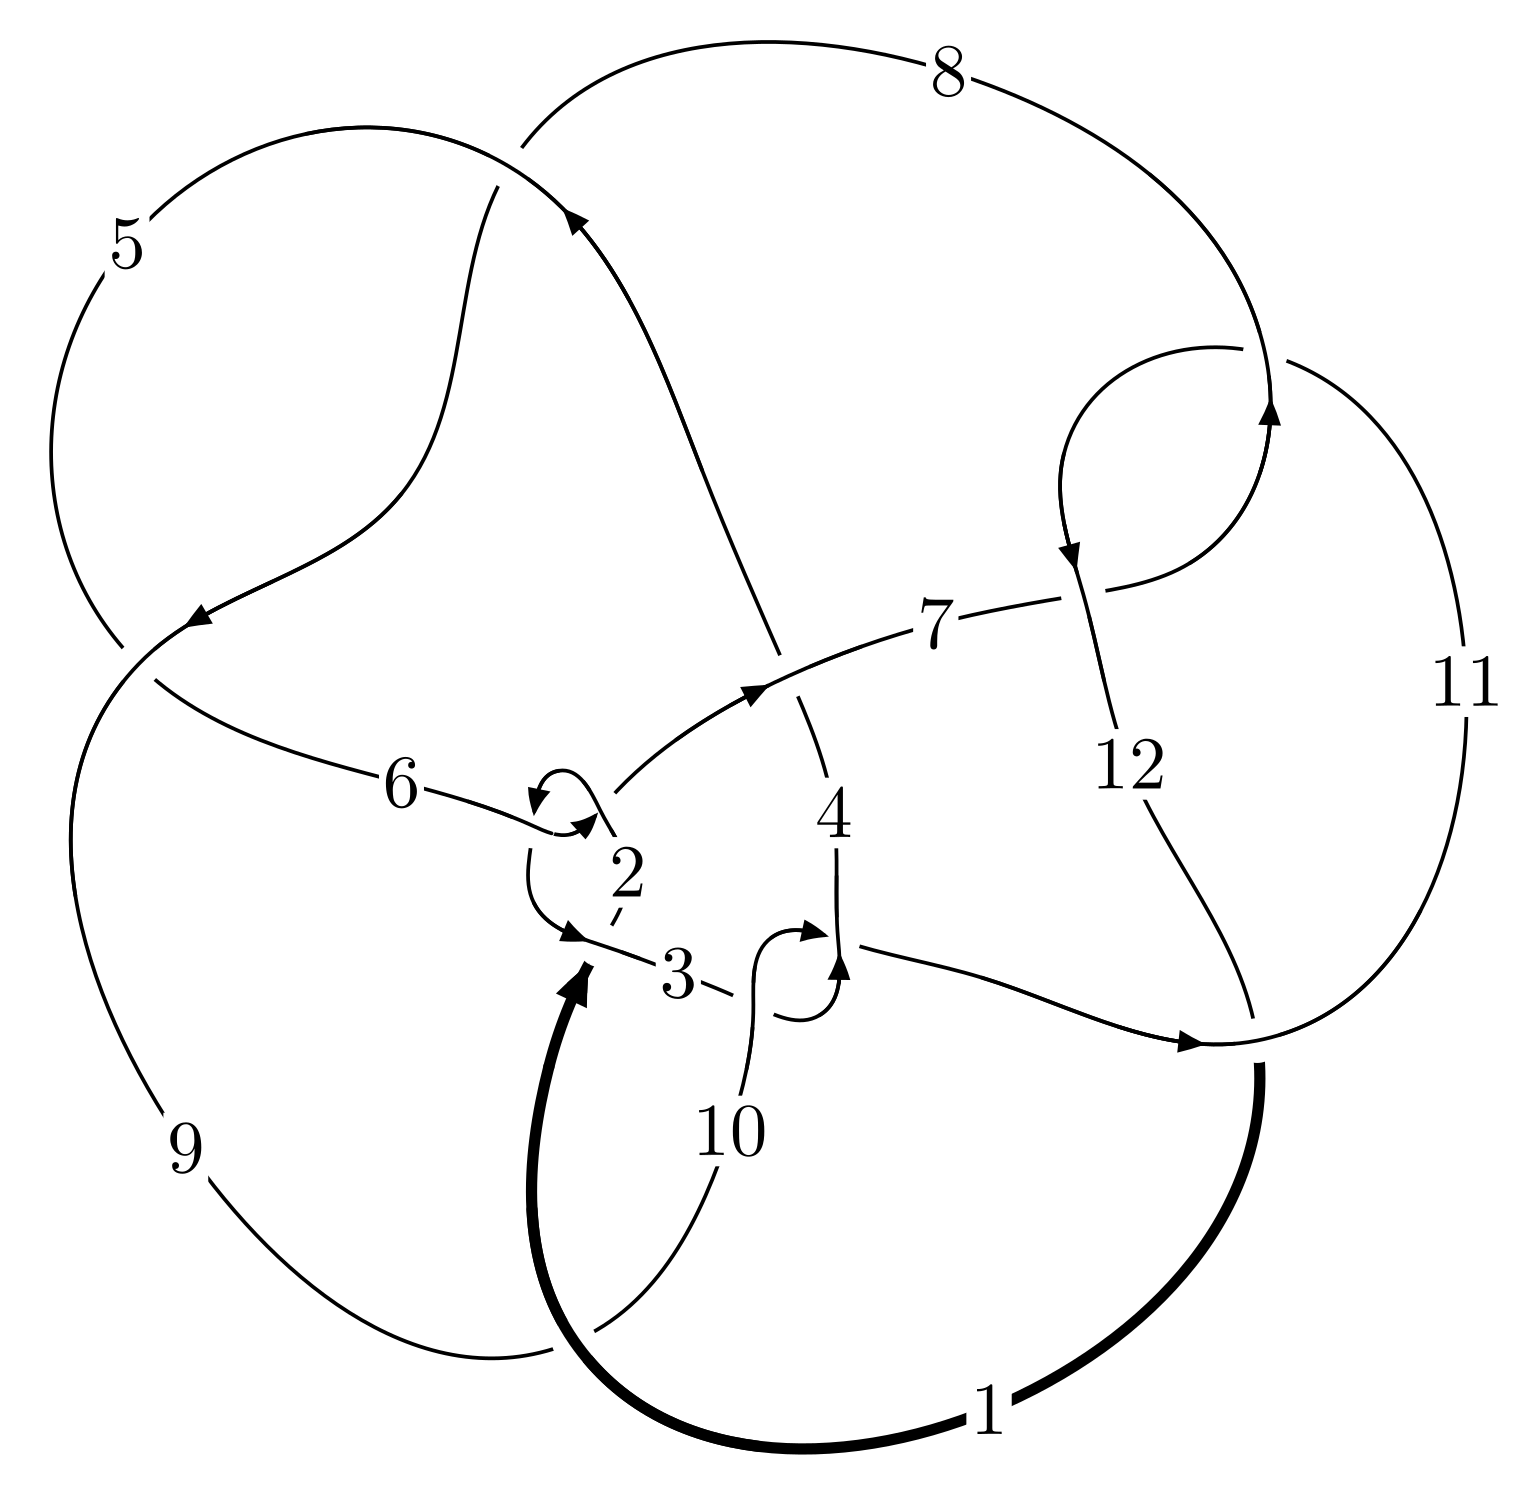
\includegraphics[width=112pt]{../../../GIT/diagram.site/diagram/png/1228_12a_0427.png}\\
\ \ \ A knot diagram\footnotemark}&
\allowdisplaybreaks
\textbf{Linearized knot diagam} \\
\cline{2-2}
 &
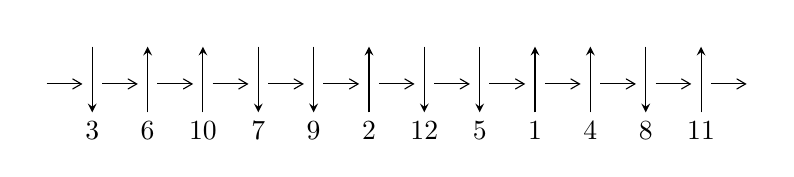
\begin{tikzpicture}[x=20pt, y=17pt]
	% nodes
	\node (C0) at (0, 0) {};
	\node (C1) at (1, 0) {};
	\node (C1U) at (1, +1) {};
	\node (C1D) at (1, -1) {3};

	\node (C2) at (2, 0) {};
	\node (C2U) at (2, +1) {};
	\node (C2D) at (2, -1) {6};

	\node (C3) at (3, 0) {};
	\node (C3U) at (3, +1) {};
	\node (C3D) at (3, -1) {10};

	\node (C4) at (4, 0) {};
	\node (C4U) at (4, +1) {};
	\node (C4D) at (4, -1) {7};

	\node (C5) at (5, 0) {};
	\node (C5U) at (5, +1) {};
	\node (C5D) at (5, -1) {9};

	\node (C6) at (6, 0) {};
	\node (C6U) at (6, +1) {};
	\node (C6D) at (6, -1) {2};

	\node (C7) at (7, 0) {};
	\node (C7U) at (7, +1) {};
	\node (C7D) at (7, -1) {12};

	\node (C8) at (8, 0) {};
	\node (C8U) at (8, +1) {};
	\node (C8D) at (8, -1) {5};

	\node (C9) at (9, 0) {};
	\node (C9U) at (9, +1) {};
	\node (C9D) at (9, -1) {1};

	\node (C10) at (10, 0) {};
	\node (C10U) at (10, +1) {};
	\node (C10D) at (10, -1) {4};

	\node (C11) at (11, 0) {};
	\node (C11U) at (11, +1) {};
	\node (C11D) at (11, -1) {8};

	\node (C12) at (12, 0) {};
	\node (C12U) at (12, +1) {};
	\node (C12D) at (12, -1) {11};
	\node (C13) at (13, 0) {};

	% arrows
	\draw[->,>={angle 60}]
	(C0) edge (C1) (C1) edge (C2) (C2) edge (C3) (C3) edge (C4) (C4) edge (C5) (C5) edge (C6) (C6) edge (C7) (C7) edge (C8) (C8) edge (C9) (C9) edge (C10) (C10) edge (C11) (C11) edge (C12) (C12) edge (C13) ;	\draw[->,>=stealth]
	(C1U) edge (C1D) (C2D) edge (C2U) (C3D) edge (C3U) (C4U) edge (C4D) (C5U) edge (C5D) (C6D) edge (C6U) (C7U) edge (C7D) (C8U) edge (C8D) (C9D) edge (C9U) (C10D) edge (C10U) (C11U) edge (C11D) (C12D) edge (C12U) ;
	\end{tikzpicture} \\
\hhline{~~} \\& 
\textbf{Solving Sequence} \\ \cline{2-2} 
 &
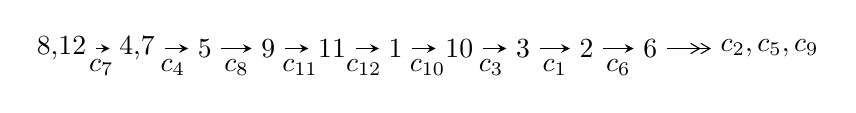
\begin{tikzpicture}[x=23pt, y=7pt]
	% node
	\node (A0) at (-1/8, 0) {8,12};
	\node (A1) at (17/16, 0) {4,7};
	\node (A2) at (17/8, 0) {5};
	\node (A3) at (25/8, 0) {9};
	\node (A4) at (33/8, 0) {11};
	\node (A5) at (41/8, 0) {1};
	\node (A6) at (49/8, 0) {10};
	\node (A7) at (57/8, 0) {3};
	\node (A8) at (65/8, 0) {2};
	\node (A9) at (73/8, 0) {6};
	\node (C1) at (1/2, -1) {$c_{7}$};
	\node (C2) at (13/8, -1) {$c_{4}$};
	\node (C3) at (21/8, -1) {$c_{8}$};
	\node (C4) at (29/8, -1) {$c_{11}$};
	\node (C5) at (37/8, -1) {$c_{12}$};
	\node (C6) at (45/8, -1) {$c_{10}$};
	\node (C7) at (53/8, -1) {$c_{3}$};
	\node (C8) at (61/8, -1) {$c_{1}$};
	\node (C9) at (69/8, -1) {$c_{6}$};
	\node (A10) at (11, 0) {$c_{2},c_{5},c_{9}$};

	% edge
	\draw[->,>=stealth]	
	(A0) edge (A1) (A1) edge (A2) (A2) edge (A3) (A3) edge (A4) (A4) edge (A5) (A5) edge (A6) (A6) edge (A7) (A7) edge (A8) (A8) edge (A9) ;
	\draw[->>,>={angle 60}]	
	(A9) edge (A10);
\end{tikzpicture} \\ 

\end{tabular} \\

\footnotetext{
The image of knot diagram is generated by the software ``\textbf{Draw programme}" developed by Andrew Bartholomew(\url{http://www.layer8.co.uk/maths/draw/index.htm\#Running-draw}), where we modified some parts for our purpose(\url{https://github.com/CATsTAILs/LinksPainter}).
}\phantom \\ \newline 
\centering \textbf{Ideals for irreducible components\footnotemark of $X_{\text{par}}$} 
 
\begin{align*}
I^u_{1}&=\langle 
575260 u^{67}+2605705 u^{66}+\cdots+248832 b-26005926,\\
\phantom{I^u_{1}}&\phantom{= \langle  }563467900 u^{67}+2831326125 u^{66}+\cdots+212253696 a+11136298543,\\
\phantom{I^u_{1}}&\phantom{= \langle  }5 u^{68}+30 u^{67}+\cdots+5054 u+853\rangle \\
I^u_{2}&=\langle 
- a^2 u+a u+b-2 a+2,\;a^3-2 a^2 u+2 a^2+a u-2 a+3 u-1,\;u^2- u+1\rangle \\
I^u_{3}&=\langle 
u^4+b,\;- u^2+a-1,\;u^5+u^3+u+1\rangle \\
I^u_{4}&=\langle 
b+u,\;a+u,\;u^5+u^3+u-1\rangle \\
I^u_{5}&=\langle 
b^2 a u-2 a^2 b u+a^3 u+b^3-3 b^2 a+3 a^2 b- a^3+2 b u- a u- a+u-1,\;u^2- u+1\rangle \\
I^u_{6}&=\langle 
b a u- a^2 u+b^2-2 b a+b u+a^2- a u- b+u,\;u^2- u+1\rangle \\
I^u_{7}&=\langle 
u^2 a+a u+b,\;u^3 a+u^2 a+a u-1\rangle \\
I^u_{8}&=\langle 
b- a- u+1,\;u^2- u+1\rangle \\
\\
I^v_{1}&=\langle 
a,\;b^6-2 b^4- b^3+b^2+b+1,\;v-1\rangle \\
\end{align*}
\raggedright * 5 irreducible components of $\dim_{\mathbb{C}}=0$, with total 90 representations.\\
\raggedright * 4 irreducible components of $\dim_{\mathbb{C}}=1$ \\
\footnotetext{All coefficients of polynomials are rational numbers. But the coefficients are sometimes approximated in decimal forms when there is not enough margin.}
\newpage
\renewcommand{\arraystretch}{1}
\centering \section*{I. $I^u_{1}= \langle 5.75\times10^{5} u^{67}+2.61\times10^{6} u^{66}+\cdots+2.49\times10^{5} b-2.60\times10^{7},\;5.63\times10^{8} u^{67}+2.83\times10^{9} u^{66}+\cdots+2.12\times10^{8} a+1.11\times10^{10},\;5 u^{68}+30 u^{67}+\cdots+5054 u+853 \rangle$}
\flushleft \textbf{(i) Arc colorings}\\
\begin{tabular}{m{7pt} m{180pt} m{7pt} m{180pt} }
\flushright $a_{8}=$&$\begin{pmatrix}1\\0\end{pmatrix}$ \\
\flushright $a_{12}=$&$\begin{pmatrix}0\\u\end{pmatrix}$ \\
\flushright $a_{4}=$&$\begin{pmatrix}-2.65469 u^{67}-13.3393 u^{66}+\cdots-582.171 u-52.4669\\-2.31184 u^{67}-10.4717 u^{66}+\cdots+255.745 u+104.512\end{pmatrix}$ \\
\flushright $a_{7}=$&$\begin{pmatrix}1\\- u^2\end{pmatrix}$ \\
\flushright $a_{5}=$&$\begin{pmatrix}-1.24736 u^{67}-3.35352 u^{66}+\cdots+1325.95 u+284.669\\1.92813 u^{67}+11.8675 u^{66}+\cdots+2054.31 u+367.547\end{pmatrix}$ \\
\flushright $a_{9}=$&$\begin{pmatrix}-0.313259 u^{67}-1.69428 u^{66}+\cdots-190.456 u-28.1702\\0.0108507 u^{67}+0.221354 u^{66}+\cdots+85.6145 u+16.6233\end{pmatrix}$ \\
\flushright $a_{11}=$&$\begin{pmatrix}u\\u\end{pmatrix}$ \\
\flushright $a_{1}=$&$\begin{pmatrix}u^3\\u^3+u\end{pmatrix}$ \\
\flushright $a_{10}=$&$\begin{pmatrix}0.103137 u^{67}+0.458229 u^{66}+\cdots-55.5265 u-13.1298\\0.158691 u^{67}+0.674371 u^{66}+\cdots-92.1597 u-23.0834\end{pmatrix}$ \\
\flushright $a_{3}=$&$\begin{pmatrix}-1.97519 u^{67}-5.35349 u^{66}+\cdots+1993.77 u+439.517\\2.40346 u^{67}+18.6888 u^{66}+\cdots+4616.08 u+863.329\end{pmatrix}$ \\
\flushright $a_{2}=$&$\begin{pmatrix}3.36495 u^{67}+16.0548 u^{66}+\cdots+184.845 u-49.3617\\1.33590 u^{67}+2.51799 u^{66}+\cdots-2210.43 u-464.485\end{pmatrix}$ \\
\flushright $a_{6}=$&$\begin{pmatrix}2.83094 u^{67}+10.9767 u^{66}+\cdots-906.631 u-247.880\\-2.22960 u^{67}-16.9831 u^{66}+\cdots-4002.13 u-746.999\end{pmatrix}$\\&\end{tabular}
\flushleft \textbf{(ii) Obstruction class $= -1$}\\~\\
\flushleft \textbf{(iii) Cusp Shapes $= -\frac{327295}{186624} u^{67}-\frac{1808905}{124416} u^{66}+\cdots-\frac{177580613}{46656} u-\frac{269328401}{373248}$}\\~\\
\newpage\renewcommand{\arraystretch}{1}
\flushleft \textbf{(iv) u-Polynomials at the component}\newline \\
\begin{tabular}{m{50pt}|m{274pt}}
Crossings & \hspace{64pt}u-Polynomials at each crossing \\
\hline $$\begin{aligned}c_{1}\end{aligned}$$&$\begin{aligned}
&25(25 u^{68}+680 u^{67}+\cdots+7437476 u+727609)
\end{aligned}$\\
\hline $$\begin{aligned}c_{2},c_{6}\end{aligned}$$&$\begin{aligned}
&5(5 u^{68}+30 u^{67}+\cdots+5054 u+853)
\end{aligned}$\\
\hline $$\begin{aligned}c_{3},c_{10}\end{aligned}$$&$\begin{aligned}
&81(81 u^{68}+648 u^{67}+\cdots+29832 u+4477)
\end{aligned}$\\
\hline $$\begin{aligned}c_{4}\end{aligned}$$&$\begin{aligned}
&64(64 u^{68}-256 u^{67}+\cdots-4.94845\times10^{7} u+9687600)
\end{aligned}$\\
\hline $$\begin{aligned}c_{5},c_{8}\end{aligned}$$&$\begin{aligned}
&81(81 u^{68}-648 u^{67}+\cdots-29832 u+4477)
\end{aligned}$\\
\hline $$\begin{aligned}c_{7},c_{11}\end{aligned}$$&$\begin{aligned}
&5(5 u^{68}-30 u^{67}+\cdots-5054 u+853)
\end{aligned}$\\
\hline $$\begin{aligned}c_{9}\end{aligned}$$&$\begin{aligned}
&64(64 u^{68}+256 u^{67}+\cdots+4.94845\times10^{7} u+9687600)
\end{aligned}$\\
\hline $$\begin{aligned}c_{12}\end{aligned}$$&$\begin{aligned}
&25(25 u^{68}-680 u^{67}+\cdots-7437476 u+727609)
\end{aligned}$\\
\hline
\end{tabular}\\~\\
\newpage\renewcommand{\arraystretch}{1}
\flushleft \textbf{(v) Riley Polynomials at the component}\newline \\
\begin{tabular}{m{50pt}|m{274pt}}
Crossings & \hspace{64pt}Riley Polynomials at each crossing \\
\hline $$\begin{aligned}c_{1},c_{12}\end{aligned}$$&$\begin{aligned}
&625\\
&\cdot(625 y^{68}+16300 y^{67}+\cdots+11609525524248 y+529414856881)
\end{aligned}$\\
\hline $$\begin{aligned}c_{2},c_{6},c_{7}\\c_{11}\end{aligned}$$&$\begin{aligned}
&25(25 y^{68}+680 y^{67}+\cdots+7437476 y+727609)
\end{aligned}$\\
\hline $$\begin{aligned}c_{3},c_{5},c_{8}\\c_{10}\end{aligned}$$&$\begin{aligned}
&6561(6561 y^{68}-279936 y^{67}+\cdots-3.61575\times10^{7} y+2.00435\times10^{7})
\end{aligned}$\\
\hline $$\begin{aligned}c_{4},c_{9}\end{aligned}$$&$\begin{aligned}
&4096\\
&\cdot(4096 y^{68}-8192 y^{67}+\cdots-815469037963200 y+93849593760000)
\end{aligned}$\\
\hline
\end{tabular}\\~\\
\newpage\flushleft \textbf{(vi) Complex Volumes and Cusp Shapes}
$$\begin{array}{c|c|c}  
\text{Solutions to }I^u_{1}& \I (\text{vol} + \sqrt{-1}CS) & \text{Cusp shape}\\
 \hline 
\begin{aligned}
u &= \phantom{-}0.702519 + 0.717277 I \\
a &= -0.75644 - 1.31522 I \\
b &= -1.296900 - 0.451791 I\end{aligned}
 & \phantom{-}1.29111 - 5.34461 I & \phantom{-0.000000 } 0 \\ \hline\begin{aligned}
u &= \phantom{-}0.702519 - 0.717277 I \\
a &= -0.75644 + 1.31522 I \\
b &= -1.296900 + 0.451791 I\end{aligned}
 & \phantom{-}1.29111 + 5.34461 I & \phantom{-0.000000 } 0 \\ \hline\begin{aligned}
u &= -0.772722 + 0.614454 I \\
a &= -0.904625 - 0.687185 I \\
b &= -0.34299 - 1.42396 I\end{aligned}
 & -3.93086 - 2.25762 I & \phantom{-0.000000 } 0 \\ \hline\begin{aligned}
u &= -0.772722 - 0.614454 I \\
a &= -0.904625 + 0.687185 I \\
b &= -0.34299 + 1.42396 I\end{aligned}
 & -3.93086 + 2.25762 I & \phantom{-0.000000 } 0 \\ \hline\begin{aligned}
u &= -0.787880 + 0.588901 I \\
a &= \phantom{-}1.094050 + 0.575479 I \\
b &= \phantom{-}0.45000 + 1.53766 I\end{aligned}
 & -5.97017 - 7.33663 I & \phantom{-0.000000 } 0 \\ \hline\begin{aligned}
u &= -0.787880 - 0.588901 I \\
a &= \phantom{-}1.094050 - 0.575479 I \\
b &= \phantom{-}0.45000 - 1.53766 I\end{aligned}
 & -5.97017 + 7.33663 I & \phantom{-0.000000 } 0 \\ \hline\begin{aligned}
u &= \phantom{-}0.112405 + 1.036780 I \\
a &= -0.685771 - 0.811514 I \\
b &= -0.008091 - 0.465537 I\end{aligned}
 & -0.02177 - 6.74730 I & \phantom{-0.000000 } 0 \\ \hline\begin{aligned}
u &= \phantom{-}0.112405 - 1.036780 I \\
a &= -0.685771 + 0.811514 I \\
b &= -0.008091 + 0.465537 I\end{aligned}
 & -0.02177 + 6.74730 I & \phantom{-0.000000 } 0 \\ \hline\begin{aligned}
u &= -0.833820 + 0.630175 I \\
a &= \phantom{-}0.718590 + 0.298717 I \\
b &= \phantom{-}0.549137 + 1.181960 I\end{aligned}
 & -8.97416 + 0.22766 I & \phantom{-0.000000 } 0 \\ \hline\begin{aligned}
u &= -0.833820 - 0.630175 I \\
a &= \phantom{-}0.718590 - 0.298717 I \\
b &= \phantom{-}0.549137 - 1.181960 I\end{aligned}
 & -8.97416 - 0.22766 I & \phantom{-0.000000 } 0\\
 \hline 
 \end{array}$$\newpage$$\begin{array}{c|c|c}  
\text{Solutions to }I^u_{1}& \I (\text{vol} + \sqrt{-1}CS) & \text{Cusp shape}\\
 \hline 
\begin{aligned}
u &= \phantom{-}0.078667 + 0.947690 I \\
a &= \phantom{-}0.769173 + 0.818647 I \\
b &= \phantom{-}0.215986 + 0.247360 I\end{aligned}
 & \phantom{-}1.67199 - 2.07344 I & \phantom{-}4.37435 + 4.03078 I \\ \hline\begin{aligned}
u &= \phantom{-}0.078667 - 0.947690 I \\
a &= \phantom{-}0.769173 - 0.818647 I \\
b &= \phantom{-}0.215986 - 0.247360 I\end{aligned}
 & \phantom{-}1.67199 + 2.07344 I & \phantom{-}4.37435 - 4.03078 I \\ \hline\begin{aligned}
u &= \phantom{-}0.937214 + 0.495255 I \\
a &= \phantom{-}0.95339 - 1.23785 I \\
b &= -0.408666 - 1.113570 I\end{aligned}
 & -1.95572 + 13.26270 I & \phantom{-0.000000 } 0 \\ \hline\begin{aligned}
u &= \phantom{-}0.937214 - 0.495255 I \\
a &= \phantom{-}0.95339 + 1.23785 I \\
b &= -0.408666 + 1.113570 I\end{aligned}
 & -1.95572 - 13.26270 I & \phantom{-0.000000 } 0 \\ \hline\begin{aligned}
u &= \phantom{-}0.984482 + 0.423718 I \\
a &= \phantom{-}0.934550 - 0.721368 I \\
b &= -0.123632 - 0.785388 I\end{aligned}
 & -7.11233 + 4.71108 I & \phantom{-0.000000 } 0 \\ \hline\begin{aligned}
u &= \phantom{-}0.984482 - 0.423718 I \\
a &= \phantom{-}0.934550 + 0.721368 I \\
b &= -0.123632 + 0.785388 I\end{aligned}
 & -7.11233 - 4.71108 I & \phantom{-0.000000 } 0 \\ \hline\begin{aligned}
u &= \phantom{-}0.957820 + 0.502893 I \\
a &= -0.811297 + 1.154980 I \\
b &= \phantom{-}0.446758 + 0.985756 I\end{aligned}
 & \phantom{-0.000000 -}7.23221 I & \phantom{-0.000000 } 0 \\ \hline\begin{aligned}
u &= \phantom{-}0.957820 - 0.502893 I \\
a &= -0.811297 - 1.154980 I \\
b &= \phantom{-}0.446758 - 0.985756 I\end{aligned}
 & \phantom{-0.000000 } -7.23221 I & \phantom{-0.000000 } 0 \\ \hline\begin{aligned}
u &= \phantom{-}0.526643 + 0.956182 I \\
a &= \phantom{-}0.65049 + 1.37033 I \\
b &= \phantom{-}1.06139 + 1.06704 I\end{aligned}
 & -0.45309 - 3.04384 I & \phantom{-0.000000 } 0 \\ \hline\begin{aligned}
u &= \phantom{-}0.526643 - 0.956182 I \\
a &= \phantom{-}0.65049 - 1.37033 I \\
b &= \phantom{-}1.06139 - 1.06704 I\end{aligned}
 & -0.45309 + 3.04384 I & \phantom{-0.000000 } 0\\
 \hline 
 \end{array}$$\newpage$$\begin{array}{c|c|c}  
\text{Solutions to }I^u_{1}& \I (\text{vol} + \sqrt{-1}CS) & \text{Cusp shape}\\
 \hline 
\begin{aligned}
u &= -0.749817 + 0.415369 I \\
a &= -1.04809 - 1.17549 I \\
b &= \phantom{-}0.620776 - 1.056180 I\end{aligned}
 & \phantom{-}2.68807 - 7.69227 I & \phantom{-}0.67631 + 5.85863 I \\ \hline\begin{aligned}
u &= -0.749817 - 0.415369 I \\
a &= -1.04809 + 1.17549 I \\
b &= \phantom{-}0.620776 + 1.056180 I\end{aligned}
 & \phantom{-}2.68807 + 7.69227 I & \phantom{-}0.67631 - 5.85863 I \\ \hline\begin{aligned}
u &= -0.670154 + 0.937244 I \\
a &= -1.45327 + 0.06264 I \\
b &= -1.234960 - 0.202287 I\end{aligned}
 & -1.29111 + 5.34461 I & \phantom{-0.000000 } 0 \\ \hline\begin{aligned}
u &= -0.670154 - 0.937244 I \\
a &= -1.45327 - 0.06264 I \\
b &= -1.234960 + 0.202287 I\end{aligned}
 & -1.29111 - 5.34461 I & \phantom{-0.000000 } 0 \\ \hline\begin{aligned}
u &= -0.117684 + 1.148120 I \\
a &= \phantom{-}0.066271 + 0.344259 I \\
b &= -0.348380 - 0.848238 I\end{aligned}
 & \phantom{-}7.75434 - 5.46492 I & \phantom{-0.000000 } 0 \\ \hline\begin{aligned}
u &= -0.117684 - 1.148120 I \\
a &= \phantom{-}0.066271 - 0.344259 I \\
b &= -0.348380 + 0.848238 I\end{aligned}
 & \phantom{-}7.75434 + 5.46492 I & \phantom{-0.000000 } 0 \\ \hline\begin{aligned}
u &= -0.753289 + 0.380335 I \\
a &= \phantom{-}0.98818 + 1.05811 I \\
b &= -0.609854 + 0.844847 I\end{aligned}
 & \phantom{-}3.93086 - 2.25762 I & \phantom{-}3.33892 + 0.57210 I \\ \hline\begin{aligned}
u &= -0.753289 - 0.380335 I \\
a &= \phantom{-}0.98818 - 1.05811 I \\
b &= -0.609854 - 0.844847 I\end{aligned}
 & \phantom{-}3.93086 + 2.25762 I & \phantom{-}3.33892 - 0.57210 I \\ \hline\begin{aligned}
u &= -0.341284 + 0.760500 I \\
a &= -2.29641 - 0.77204 I \\
b &= -1.73365 - 0.13982 I\end{aligned}
 & \phantom{-}0.45309 + 3.04384 I & \phantom{-}3.47317 + 0.77959 I \\ \hline\begin{aligned}
u &= -0.341284 - 0.760500 I \\
a &= -2.29641 + 0.77204 I \\
b &= -1.73365 + 0.13982 I\end{aligned}
 & \phantom{-}0.45309 - 3.04384 I & \phantom{-}3.47317 - 0.77959 I\\
 \hline 
 \end{array}$$\newpage$$\begin{array}{c|c|c}  
\text{Solutions to }I^u_{1}& \I (\text{vol} + \sqrt{-1}CS) & \text{Cusp shape}\\
 \hline 
\begin{aligned}
u &= -0.145225 + 0.813062 I \\
a &= \phantom{-}1.28772 + 0.60761 I \\
b &= \phantom{-}0.749993 - 0.175588 I\end{aligned}
 & \phantom{-}1.65241 - 1.05941 I & \phantom{-}6.63964 + 4.57024 I \\ \hline\begin{aligned}
u &= -0.145225 - 0.813062 I \\
a &= \phantom{-}1.28772 - 0.60761 I \\
b &= \phantom{-}0.749993 + 0.175588 I\end{aligned}
 & \phantom{-}1.65241 + 1.05941 I & \phantom{-}6.63964 - 4.57024 I \\ \hline\begin{aligned}
u &= \phantom{-}0.780665 + 0.269621 I \\
a &= \phantom{-}1.108650 + 0.142041 I \\
b &= \phantom{-}0.637811 - 0.389139 I\end{aligned}
 & -4.47467 - 4.39199 I & -7.74935 + 3.75955 I \\ \hline\begin{aligned}
u &= \phantom{-}0.780665 - 0.269621 I \\
a &= \phantom{-}1.108650 - 0.142041 I \\
b &= \phantom{-}0.637811 + 0.389139 I\end{aligned}
 & -4.47467 + 4.39199 I & -7.74935 - 3.75955 I \\ \hline\begin{aligned}
u &= -0.132701 + 1.176080 I \\
a &= \phantom{-}0.023962 - 0.238727 I \\
b &= \phantom{-}0.328720 + 0.927847 I\end{aligned}
 & \phantom{-}8.97416 + 0.22766 I & \phantom{-0.000000 } 0 \\ \hline\begin{aligned}
u &= -0.132701 - 1.176080 I \\
a &= \phantom{-}0.023962 + 0.238727 I \\
b &= \phantom{-}0.328720 - 0.927847 I\end{aligned}
 & \phantom{-}8.97416 - 0.22766 I & \phantom{-0.000000 } 0 \\ \hline\begin{aligned}
u &= -0.567585 + 1.053430 I \\
a &= -1.51541 - 0.77084 I \\
b &= -1.55197 - 1.72836 I\end{aligned}
 & \phantom{-}0.02177 + 6.74730 I & \phantom{-0.000000 } 0 \\ \hline\begin{aligned}
u &= -0.567585 - 1.053430 I \\
a &= -1.51541 + 0.77084 I \\
b &= -1.55197 + 1.72836 I\end{aligned}
 & \phantom{-}0.02177 - 6.74730 I & \phantom{-0.000000 } 0 \\ \hline\begin{aligned}
u &= -1.059300 + 0.560745 I \\
a &= \phantom{-}0.104792 - 0.286003 I \\
b &= \phantom{-}0.754560 + 0.357556 I\end{aligned}
 & -2.18567 + 7.77249 I & \phantom{-0.000000 } 0 \\ \hline\begin{aligned}
u &= -1.059300 - 0.560745 I \\
a &= \phantom{-}0.104792 + 0.286003 I \\
b &= \phantom{-}0.754560 - 0.357556 I\end{aligned}
 & -2.18567 - 7.77249 I & \phantom{-0.000000 } 0\\
 \hline 
 \end{array}$$\newpage$$\begin{array}{c|c|c}  
\text{Solutions to }I^u_{1}& \I (\text{vol} + \sqrt{-1}CS) & \text{Cusp shape}\\
 \hline 
\begin{aligned}
u &= -0.662387 + 1.025070 I \\
a &= -1.40530 - 0.89343 I \\
b &= -0.72294 - 1.44985 I\end{aligned}
 & -2.68807 + 7.69227 I & \phantom{-0.000000 } 0 \\ \hline\begin{aligned}
u &= -0.662387 - 1.025070 I \\
a &= -1.40530 + 0.89343 I \\
b &= -0.72294 + 1.44985 I\end{aligned}
 & -2.68807 - 7.69227 I & \phantom{-0.000000 } 0 \\ \hline\begin{aligned}
u &= -0.663727 + 1.037980 I \\
a &= \phantom{-}1.38765 + 1.08315 I \\
b &= \phantom{-}0.54606 + 1.68325 I\end{aligned}
 & -4.61883 + 12.81070 I & \phantom{-0.000000 } 0 \\ \hline\begin{aligned}
u &= -0.663727 - 1.037980 I \\
a &= \phantom{-}1.38765 - 1.08315 I \\
b &= \phantom{-}0.54606 - 1.68325 I\end{aligned}
 & -4.61883 - 12.81070 I & \phantom{-0.000000 } 0 \\ \hline\begin{aligned}
u &= -0.603158 + 1.083480 I \\
a &= -1.75432 - 0.31678 I \\
b &= -1.84792 - 1.60763 I\end{aligned}
 & \phantom{-}4.61883 + 12.81070 I & \phantom{-0.000000 } 0 \\ \hline\begin{aligned}
u &= -0.603158 - 1.083480 I \\
a &= -1.75432 + 0.31678 I \\
b &= -1.84792 + 1.60763 I\end{aligned}
 & \phantom{-}4.61883 - 12.81070 I & \phantom{-0.000000 } 0 \\ \hline\begin{aligned}
u &= -0.692945 + 1.028870 I \\
a &= \phantom{-}1.002200 + 0.844351 I \\
b &= \phantom{-}0.244445 + 1.103960 I\end{aligned}
 & -7.75434 + 5.46492 I & \phantom{-0.000000 } 0 \\ \hline\begin{aligned}
u &= -0.692945 - 1.028870 I \\
a &= \phantom{-}1.002200 - 0.844351 I \\
b &= \phantom{-}0.244445 - 1.103960 I\end{aligned}
 & -7.75434 - 5.46492 I & \phantom{-0.000000 } 0 \\ \hline\begin{aligned}
u &= -0.599314 + 0.464063 I \\
a &= -1.33435 - 1.16820 I \\
b &= -0.107178 - 1.031260 I\end{aligned}
 & -1.67199 - 2.07344 I & -4.37435 + 4.03078 I \\ \hline\begin{aligned}
u &= -0.599314 - 0.464063 I \\
a &= -1.33435 + 1.16820 I \\
b &= -0.107178 + 1.031260 I\end{aligned}
 & -1.67199 + 2.07344 I & -4.37435 - 4.03078 I\\
 \hline 
 \end{array}$$\newpage$$\begin{array}{c|c|c}  
\text{Solutions to }I^u_{1}& \I (\text{vol} + \sqrt{-1}CS) & \text{Cusp shape}\\
 \hline 
\begin{aligned}
u &= -0.595289 + 1.091030 I \\
a &= \phantom{-}1.59309 + 0.27206 I \\
b &= \phantom{-}1.76899 + 1.48931 I\end{aligned}
 & \phantom{-}5.97017 + 7.33663 I & \phantom{-0.000000 } 0 \\ \hline\begin{aligned}
u &= -0.595289 - 1.091030 I \\
a &= \phantom{-}1.59309 - 0.27206 I \\
b &= \phantom{-}1.76899 - 1.48931 I\end{aligned}
 & \phantom{-}5.97017 - 7.33663 I & \phantom{-0.000000 } 0 \\ \hline\begin{aligned}
u &= -0.532947 + 1.124330 I \\
a &= \phantom{-}0.912459 + 0.425272 I \\
b &= \phantom{-}1.19050 + 1.36318 I\end{aligned}
 & \phantom{-}4.47467 + 4.39199 I & \phantom{-0.000000 } 0 \\ \hline\begin{aligned}
u &= -0.532947 - 1.124330 I \\
a &= \phantom{-}0.912459 - 0.425272 I \\
b &= \phantom{-}1.19050 - 1.36318 I\end{aligned}
 & \phantom{-}4.47467 - 4.39199 I & \phantom{-0.000000 } 0 \\ \hline\begin{aligned}
u &= -0.029081 + 1.297740 I \\
a &= -0.435981 - 0.038934 I \\
b &= -0.178672 - 1.072860 I\end{aligned}
 & \phantom{-}4.86026 + 10.75690 I & \phantom{-0.000000 } 0 \\ \hline\begin{aligned}
u &= -0.029081 - 1.297740 I \\
a &= -0.435981 + 0.038934 I \\
b &= -0.178672 + 1.072860 I\end{aligned}
 & \phantom{-}4.86026 - 10.75690 I & \phantom{-0.000000 } 0 \\ \hline\begin{aligned}
u &= -0.073579 + 1.312560 I \\
a &= \phantom{-}0.338952 + 0.014268 I \\
b &= \phantom{-}0.224066 + 1.023900 I\end{aligned}
 & \phantom{-}7.11233 + 4.71108 I & \phantom{-0.000000 } 0 \\ \hline\begin{aligned}
u &= -0.073579 - 1.312560 I \\
a &= \phantom{-}0.338952 - 0.014268 I \\
b &= \phantom{-}0.224066 - 1.023900 I\end{aligned}
 & \phantom{-}7.11233 - 4.71108 I & \phantom{-0.000000 } 0 \\ \hline\begin{aligned}
u &= \phantom{-}0.687648 + 1.131730 I \\
a &= \phantom{-}1.67548 - 0.61053 I \\
b &= \phantom{-}1.85706 - 1.75220 I\end{aligned}
 & \phantom{-0.000000 } -19.2093 I & \phantom{-0.000000 } 0 \\ \hline\begin{aligned}
u &= \phantom{-}0.687648 - 1.131730 I \\
a &= \phantom{-}1.67548 + 0.61053 I \\
b &= \phantom{-}1.85706 + 1.75220 I\end{aligned}
 & \phantom{-0.000000 -}19.2093 I & \phantom{-0.000000 } 0\\
 \hline 
 \end{array}$$\newpage$$\begin{array}{c|c|c}  
\text{Solutions to }I^u_{1}& \I (\text{vol} + \sqrt{-1}CS) & \text{Cusp shape}\\
 \hline 
\begin{aligned}
u &= \phantom{-}0.696018 + 1.135630 I \\
a &= -1.57600 + 0.50092 I \\
b &= -1.79380 + 1.58426 I\end{aligned}
 & \phantom{-}1.95572 - 13.26270 I & \phantom{-0.000000 } 0 \\ \hline\begin{aligned}
u &= \phantom{-}0.696018 - 1.135630 I \\
a &= -1.57600 - 0.50092 I \\
b &= -1.79380 - 1.58426 I\end{aligned}
 & \phantom{-}1.95572 + 13.26270 I & \phantom{-0.000000 } 0 \\ \hline\begin{aligned}
u &= \phantom{-}0.458183 + 0.480361 I \\
a &= -0.807160 - 1.060200 I \\
b &= -0.930879 - 0.136305 I\end{aligned}
 & -1.65241 - 1.05941 I & -6.63964 + 4.57024 I \\ \hline\begin{aligned}
u &= \phantom{-}0.458183 - 0.480361 I \\
a &= -0.807160 + 1.060200 I \\
b &= -0.930879 + 0.136305 I\end{aligned}
 & -1.65241 + 1.05941 I & -6.63964 - 4.57024 I \\ \hline\begin{aligned}
u &= \phantom{-}0.686607 + 1.164600 I \\
a &= \phantom{-}1.238110 - 0.659956 I \\
b &= \phantom{-}1.34714 - 1.61050 I\end{aligned}
 & -4.86026 - 10.75690 I & \phantom{-0.000000 } 0 \\ \hline\begin{aligned}
u &= \phantom{-}0.686607 - 1.164600 I \\
a &= \phantom{-}1.238110 + 0.659956 I \\
b &= \phantom{-}1.34714 + 1.61050 I\end{aligned}
 & -4.86026 + 10.75690 I & \phantom{-0.000000 } 0 \\ \hline\begin{aligned}
u &= \phantom{-}0.77502 + 1.18600 I \\
a &= -0.943171 + 0.128059 I \\
b &= -1.25289 + 0.90407 I\end{aligned}
 & \phantom{-}2.18567 - 7.77249 I & \phantom{-0.000000 } 0 \\ \hline\begin{aligned}
u &= \phantom{-}0.77502 - 1.18600 I \\
a &= -0.943171 - 0.128059 I \\
b &= -1.25289 - 0.90407 I\end{aligned}
 & \phantom{-}2.18567 + 7.77249 I & \phantom{-0.000000 } 0\\
 \hline 
 \end{array}$$\newpage\newpage\renewcommand{\arraystretch}{1}
\centering \section*{II. $I^u_{2}= \langle - a^2 u+a u+b-2 a+2,\;a^3-2 a^2 u+2 a^2+a u-2 a+3 u-1,\;u^2- u+1 \rangle$}
\flushleft \textbf{(i) Arc colorings}\\
\begin{tabular}{m{7pt} m{180pt} m{7pt} m{180pt} }
\flushright $a_{8}=$&$\begin{pmatrix}1\\0\end{pmatrix}$ \\
\flushright $a_{12}=$&$\begin{pmatrix}0\\u\end{pmatrix}$ \\
\flushright $a_{4}=$&$\begin{pmatrix}a\\a^2 u- a u+2 a-2\end{pmatrix}$ \\
\flushright $a_{7}=$&$\begin{pmatrix}1\\- u+1\end{pmatrix}$ \\
\flushright $a_{5}=$&$\begin{pmatrix}- a^2 u+2\\a^2 u- a^2+a-2 u\end{pmatrix}$ \\
\flushright $a_{9}=$&$\begin{pmatrix}- a^2 u+2\\- a^2 u- a+2\end{pmatrix}$ \\
\flushright $a_{11}=$&$\begin{pmatrix}u\\u\end{pmatrix}$ \\
\flushright $a_{1}=$&$\begin{pmatrix}-1\\u-1\end{pmatrix}$ \\
\flushright $a_{10}=$&$\begin{pmatrix}-2 a^2 u+a^2- a+2 u+2\\-2 a^2 u+a u-2 a+4\end{pmatrix}$ \\
\flushright $a_{3}=$&$\begin{pmatrix}1\\- u+1\end{pmatrix}$ \\
\flushright $a_{2}=$&$\begin{pmatrix}-1\\u-1\end{pmatrix}$ \\
\flushright $a_{6}=$&$\begin{pmatrix}1\\- u+1\end{pmatrix}$\\&\end{tabular}
\flushleft \textbf{(ii) Obstruction class $= -1$}\\~\\
\flushleft \textbf{(iii) Cusp Shapes $= 4 u-2$}\\~\\
\newpage\renewcommand{\arraystretch}{1}
\flushleft \textbf{(iv) u-Polynomials at the component}\newline \\
\begin{tabular}{m{50pt}|m{274pt}}
Crossings & \hspace{64pt}u-Polynomials at each crossing \\
\hline $$\begin{aligned}c_{1},c_{2},c_{6}\end{aligned}$$&$\begin{aligned}
&u^6
\end{aligned}$\\
\hline $$\begin{aligned}c_{3},c_{5},c_{8}\\c_{9},c_{10}\end{aligned}$$&$\begin{aligned}
&u^6-2 u^4+u^3+u^2- u+1
\end{aligned}$\\
\hline $$\begin{aligned}c_{4}\end{aligned}$$&$\begin{aligned}
&u^6+4 u^5+6 u^4+3 u^3- u^2- u+1
\end{aligned}$\\
\hline $$\begin{aligned}c_{7},c_{11}\end{aligned}$$&$\begin{aligned}
&(u^2+u+1)^3
\end{aligned}$\\
\hline $$\begin{aligned}c_{12}\end{aligned}$$&$\begin{aligned}
&(u^2- u+1)^3
\end{aligned}$\\
\hline
\end{tabular}\\~\\
\newpage\renewcommand{\arraystretch}{1}
\flushleft \textbf{(v) Riley Polynomials at the component}\newline \\
\begin{tabular}{m{50pt}|m{274pt}}
Crossings & \hspace{64pt}Riley Polynomials at each crossing \\
\hline $$\begin{aligned}c_{1},c_{2},c_{6}\end{aligned}$$&$\begin{aligned}
&y^6
\end{aligned}$\\
\hline $$\begin{aligned}c_{3},c_{5},c_{8}\\c_{9},c_{10}\end{aligned}$$&$\begin{aligned}
&y^6-4 y^5+6 y^4-3 y^3- y^2+y+1
\end{aligned}$\\
\hline $$\begin{aligned}c_{4}\end{aligned}$$&$\begin{aligned}
&y^6-4 y^5+10 y^4-11 y^3+19 y^2-3 y+1
\end{aligned}$\\
\hline $$\begin{aligned}c_{7},c_{11},c_{12}\end{aligned}$$&$\begin{aligned}
&(y^2+y+1)^3
\end{aligned}$\\
\hline
\end{tabular}\\~\\
\newpage\flushleft \textbf{(vi) Complex Volumes and Cusp Shapes}
$$\begin{array}{c|c|c}  
\text{Solutions to }I^u_{2}& \I (\text{vol} + \sqrt{-1}CS) & \text{Cusp shape}\\
 \hline 
\begin{aligned}
u &= \phantom{-}0.500000 + 0.866025 I \\
a &= \phantom{-}1.137010 - 0.340420 I \\
b &= \phantom{-}0.669552 - 0.863143 I\end{aligned}
 & \phantom{-0.000000 } -2.02988 I & \phantom{-0.000000 -}0. + 3.46410 I \\ \hline\begin{aligned}
u &= \phantom{-}0.500000 + 0.866025 I \\
a &= -1.072830 + 0.640783 I \\
b &= -1.49343 + 1.84400 I\end{aligned}
 & \phantom{-0.000000 } -2.02988 I & \phantom{-0.000000 -}0. + 3.46410 I \\ \hline\begin{aligned}
u &= \phantom{-}0.500000 + 0.866025 I \\
a &= -1.06417 + 1.43169 I \\
b &= -0.176126 + 0.751194 I\end{aligned}
 & \phantom{-0.000000 } -2.02988 I & \phantom{-0.000000 -}0. + 3.46410 I \\ \hline\begin{aligned}
u &= \phantom{-}0.500000 - 0.866025 I \\
a &= \phantom{-}1.137010 + 0.340420 I \\
b &= \phantom{-}0.669552 + 0.863143 I\end{aligned}
 & \phantom{-0.000000 -}2.02988 I & \phantom{-0.000000 } 0. - 3.46410 I \\ \hline\begin{aligned}
u &= \phantom{-}0.500000 - 0.866025 I \\
a &= -1.072830 - 0.640783 I \\
b &= -1.49343 - 1.84400 I\end{aligned}
 & \phantom{-0.000000 -}2.02988 I & \phantom{-0.000000 } 0. - 3.46410 I \\ \hline\begin{aligned}
u &= \phantom{-}0.500000 - 0.866025 I \\
a &= -1.06417 - 1.43169 I \\
b &= -0.176126 - 0.751194 I\end{aligned}
 & \phantom{-0.000000 -}2.02988 I & \phantom{-0.000000 } 0. - 3.46410 I\\
 \hline 
 \end{array}$$\newpage\newpage\renewcommand{\arraystretch}{1}
\centering \section*{III. $I^u_{3}= \langle u^4+b,\;- u^2+a-1,\;u^5+u^3+u+1 \rangle$}
\flushleft \textbf{(i) Arc colorings}\\
\begin{tabular}{m{7pt} m{180pt} m{7pt} m{180pt} }
\flushright $a_{8}=$&$\begin{pmatrix}1\\0\end{pmatrix}$ \\
\flushright $a_{12}=$&$\begin{pmatrix}0\\u\end{pmatrix}$ \\
\flushright $a_{4}=$&$\begin{pmatrix}u^2+1\\- u^4\end{pmatrix}$ \\
\flushright $a_{7}=$&$\begin{pmatrix}1\\- u^2\end{pmatrix}$ \\
\flushright $a_{5}=$&$\begin{pmatrix}1\\0\end{pmatrix}$ \\
\flushright $a_{9}=$&$\begin{pmatrix}1\\0\end{pmatrix}$ \\
\flushright $a_{11}=$&$\begin{pmatrix}u\\u\end{pmatrix}$ \\
\flushright $a_{1}=$&$\begin{pmatrix}u^3\\u^3+u\end{pmatrix}$ \\
\flushright $a_{10}=$&$\begin{pmatrix}u^2+u+1\\- u^4+u\end{pmatrix}$ \\
\flushright $a_{3}=$&$\begin{pmatrix}- u\\- u\end{pmatrix}$ \\
\flushright $a_{2}=$&$\begin{pmatrix}0\\u\end{pmatrix}$ \\
\flushright $a_{6}=$&$\begin{pmatrix}1\\0\end{pmatrix}$\\&\end{tabular}
\flushleft \textbf{(ii) Obstruction class $= -1$}\\~\\
\flushleft \textbf{(iii) Cusp Shapes $= 6$}\\~\\
\newpage\renewcommand{\arraystretch}{1}
\flushleft \textbf{(iv) u-Polynomials at the component}\newline \\
\begin{tabular}{m{50pt}|m{274pt}}
Crossings & \hspace{64pt}u-Polynomials at each crossing \\
\hline $$\begin{aligned}c_{1},c_{4}\end{aligned}$$&$\begin{aligned}
&u^5+2 u^4+3 u^3+2 u^2+u-1
\end{aligned}$\\
\hline $$\begin{aligned}c_{2},c_{6},c_{7}\\c_{11}\end{aligned}$$&$\begin{aligned}
&u^5+u^3+u-1
\end{aligned}$\\
\hline $$\begin{aligned}c_{3},c_{10}\end{aligned}$$&$\begin{aligned}
&(u-1)^5
\end{aligned}$\\
\hline $$\begin{aligned}c_{5},c_{8}\end{aligned}$$&$\begin{aligned}
&u^5
\end{aligned}$\\
\hline $$\begin{aligned}c_{9}\end{aligned}$$&$\begin{aligned}
&u^5+u^3+2 u^2- u-2
\end{aligned}$\\
\hline $$\begin{aligned}c_{12}\end{aligned}$$&$\begin{aligned}
&u^5-2 u^4+3 u^3-2 u^2+u+1
\end{aligned}$\\
\hline
\end{tabular}\\~\\
\newpage\renewcommand{\arraystretch}{1}
\flushleft \textbf{(v) Riley Polynomials at the component}\newline \\
\begin{tabular}{m{50pt}|m{274pt}}
Crossings & \hspace{64pt}Riley Polynomials at each crossing \\
\hline $$\begin{aligned}c_{1},c_{4},c_{12}\end{aligned}$$&$\begin{aligned}
&y^5+2 y^4+3 y^3+6 y^2+5 y-1
\end{aligned}$\\
\hline $$\begin{aligned}c_{2},c_{6},c_{7}\\c_{11}\end{aligned}$$&$\begin{aligned}
&y^5+2 y^4+3 y^3+2 y^2+y-1
\end{aligned}$\\
\hline $$\begin{aligned}c_{3},c_{10}\end{aligned}$$&$\begin{aligned}
&(y-1)^5
\end{aligned}$\\
\hline $$\begin{aligned}c_{5},c_{8}\end{aligned}$$&$\begin{aligned}
&y^5
\end{aligned}$\\
\hline $$\begin{aligned}c_{9}\end{aligned}$$&$\begin{aligned}
&y^5+2 y^4- y^3-6 y^2+9 y-4
\end{aligned}$\\
\hline
\end{tabular}\\~\\
\newpage\flushleft \textbf{(vi) Complex Volumes and Cusp Shapes}
$$\begin{array}{c|c|c}  
\text{Solutions to }I^u_{3}& \I (\text{vol} + \sqrt{-1}CS) & \text{Cusp shape}\\
 \hline 
\begin{aligned}
u &= \phantom{-}0.707729 + 0.841955 I \\
a &= \phantom{-}0.79199 + 1.19175 I \\
b &= \phantom{-}1.37700 + 0.49579 I\end{aligned}
 & \phantom{-}1.64493\phantom{ +0.000000I} & \phantom{-}6.00000\phantom{ +0.000000I} \\ \hline\begin{aligned}
u &= \phantom{-}0.707729 - 0.841955 I \\
a &= \phantom{-}0.79199 - 1.19175 I \\
b &= \phantom{-}1.37700 - 0.49579 I\end{aligned}
 & \phantom{-}1.64493\phantom{ +0.000000I} & \phantom{-}6.00000\phantom{ +0.000000I} \\ \hline\begin{aligned}
u &= -0.389287 + 1.070680 I \\
a &= \phantom{-}0.005198 - 0.833601 I \\
b &= -0.29474 - 1.65854 I\end{aligned}
 & \phantom{-}1.64493\phantom{ +0.000000I} & \phantom{-}6.00000\phantom{ +0.000000I} \\ \hline\begin{aligned}
u &= -0.389287 - 1.070680 I \\
a &= \phantom{-}0.005198 + 0.833601 I \\
b &= -0.29474 + 1.65854 I\end{aligned}
 & \phantom{-}1.64493\phantom{ +0.000000I} & \phantom{-}6.00000\phantom{ +0.000000I} \\ \hline\begin{aligned}
u &= -0.636883\phantom{ +0.000000I} \\
a &= \phantom{-}1.40562\phantom{ +0.000000I} \\
b &= -0.164527\phantom{ +0.000000I}\end{aligned}
 & \phantom{-}1.64493\phantom{ +0.000000I} & \phantom{-}6.00000\phantom{ +0.000000I}\\
 \hline 
 \end{array}$$\newpage\newpage\renewcommand{\arraystretch}{1}
\centering \section*{IV. $I^u_{4}= \langle b+u,\;a+u,\;u^5+u^3+u-1 \rangle$}
\flushleft \textbf{(i) Arc colorings}\\
\begin{tabular}{m{7pt} m{180pt} m{7pt} m{180pt} }
\flushright $a_{8}=$&$\begin{pmatrix}1\\0\end{pmatrix}$ \\
\flushright $a_{12}=$&$\begin{pmatrix}0\\u\end{pmatrix}$ \\
\flushright $a_{4}=$&$\begin{pmatrix}- u\\- u\end{pmatrix}$ \\
\flushright $a_{7}=$&$\begin{pmatrix}1\\- u^2\end{pmatrix}$ \\
\flushright $a_{5}=$&$\begin{pmatrix}u^3\\-1\end{pmatrix}$ \\
\flushright $a_{9}=$&$\begin{pmatrix}- u^3+1\\1\end{pmatrix}$ \\
\flushright $a_{11}=$&$\begin{pmatrix}u\\u\end{pmatrix}$ \\
\flushright $a_{1}=$&$\begin{pmatrix}u^3\\u^3+u\end{pmatrix}$ \\
\flushright $a_{10}=$&$\begin{pmatrix}u\\u\end{pmatrix}$ \\
\flushright $a_{3}=$&$\begin{pmatrix}- u\\- u\end{pmatrix}$ \\
\flushright $a_{2}=$&$\begin{pmatrix}0\\u\end{pmatrix}$ \\
\flushright $a_{6}=$&$\begin{pmatrix}1\\0\end{pmatrix}$\\&\end{tabular}
\flushleft \textbf{(ii) Obstruction class $= -1$}\\~\\
\flushleft \textbf{(iii) Cusp Shapes $= -6$}\\~\\
\newpage\renewcommand{\arraystretch}{1}
\flushleft \textbf{(iv) u-Polynomials at the component}\newline \\
\begin{tabular}{m{50pt}|m{274pt}}
Crossings & \hspace{64pt}u-Polynomials at each crossing \\
\hline $$\begin{aligned}c_{1}\end{aligned}$$&$\begin{aligned}
&u^5+2 u^4+3 u^3+2 u^2+u-1
\end{aligned}$\\
\hline $$\begin{aligned}c_{2},c_{6},c_{7}\\c_{11}\end{aligned}$$&$\begin{aligned}
&u^5+u^3+u+1
\end{aligned}$\\
\hline $$\begin{aligned}c_{3},c_{10}\end{aligned}$$&$\begin{aligned}
&u^5
\end{aligned}$\\
\hline $$\begin{aligned}c_{4}\end{aligned}$$&$\begin{aligned}
&u^5+u^3-2 u^2- u+2
\end{aligned}$\\
\hline $$\begin{aligned}c_{5},c_{8}\end{aligned}$$&$\begin{aligned}
&(u+1)^5
\end{aligned}$\\
\hline $$\begin{aligned}c_{9},c_{12}\end{aligned}$$&$\begin{aligned}
&u^5-2 u^4+3 u^3-2 u^2+u+1
\end{aligned}$\\
\hline
\end{tabular}\\~\\
\newpage\renewcommand{\arraystretch}{1}
\flushleft \textbf{(v) Riley Polynomials at the component}\newline \\
\begin{tabular}{m{50pt}|m{274pt}}
Crossings & \hspace{64pt}Riley Polynomials at each crossing \\
\hline $$\begin{aligned}c_{1},c_{9},c_{12}\end{aligned}$$&$\begin{aligned}
&y^5+2 y^4+3 y^3+6 y^2+5 y-1
\end{aligned}$\\
\hline $$\begin{aligned}c_{2},c_{6},c_{7}\\c_{11}\end{aligned}$$&$\begin{aligned}
&y^5+2 y^4+3 y^3+2 y^2+y-1
\end{aligned}$\\
\hline $$\begin{aligned}c_{3},c_{10}\end{aligned}$$&$\begin{aligned}
&y^5
\end{aligned}$\\
\hline $$\begin{aligned}c_{4}\end{aligned}$$&$\begin{aligned}
&y^5+2 y^4- y^3-6 y^2+9 y-4
\end{aligned}$\\
\hline $$\begin{aligned}c_{5},c_{8}\end{aligned}$$&$\begin{aligned}
&(y-1)^5
\end{aligned}$\\
\hline
\end{tabular}\\~\\
\newpage\flushleft \textbf{(vi) Complex Volumes and Cusp Shapes}
$$\begin{array}{c|c|c}  
\text{Solutions to }I^u_{4}& \I (\text{vol} + \sqrt{-1}CS) & \text{Cusp shape}\\
 \hline 
\begin{aligned}
u &= -0.707729 + 0.841955 I \\
a &= \phantom{-}0.707729 - 0.841955 I \\
b &= \phantom{-}0.707729 - 0.841955 I\end{aligned}
 & -1.64493\phantom{ +0.000000I} & -6.00000\phantom{ +0.000000I} \\ \hline\begin{aligned}
u &= -0.707729 - 0.841955 I \\
a &= \phantom{-}0.707729 + 0.841955 I \\
b &= \phantom{-}0.707729 + 0.841955 I\end{aligned}
 & -1.64493\phantom{ +0.000000I} & -6.00000\phantom{ +0.000000I} \\ \hline\begin{aligned}
u &= \phantom{-}0.389287 + 1.070680 I \\
a &= -0.389287 - 1.070680 I \\
b &= -0.389287 - 1.070680 I\end{aligned}
 & -1.64493\phantom{ +0.000000I} & -6.00000\phantom{ +0.000000I} \\ \hline\begin{aligned}
u &= \phantom{-}0.389287 - 1.070680 I \\
a &= -0.389287 + 1.070680 I \\
b &= -0.389287 + 1.070680 I\end{aligned}
 & -1.64493\phantom{ +0.000000I} & -6.00000\phantom{ +0.000000I} \\ \hline\begin{aligned}
u &= \phantom{-}0.636883\phantom{ +0.000000I} \\
a &= -0.636883\phantom{ +0.000000I} \\
b &= -0.636883\phantom{ +0.000000I}\end{aligned}
 & -1.64493\phantom{ +0.000000I} & -6.00000\phantom{ +0.000000I}\\
 \hline 
 \end{array}$$\newpage\newpage\renewcommand{\arraystretch}{1}
\centering \section*{V. $I^u_{5}= \langle b^2 a u-2 a^2 b u+a^3 u+b^3-3 b^2 a+3 a^2 b- a^3+2 b u- a u- a+u-1,\;u^2- u+1 \rangle$}
\flushleft \textbf{(i) Arc colorings}\\
\begin{tabular}{m{7pt} m{180pt} m{7pt} m{180pt} }
\flushright $a_{8}=$&$\begin{pmatrix}1\\0\end{pmatrix}$ \\
\flushright $a_{12}=$&$\begin{pmatrix}0\\u\end{pmatrix}$ \\
\flushright $a_{4}=$&$\begin{pmatrix}a\\b\end{pmatrix}$ \\
\flushright $a_{7}=$&$\begin{pmatrix}1\\- u+1\end{pmatrix}$ \\
\flushright $a_{5}=$&$\begin{pmatrix}- a u- b+2 a\\b u- a u\end{pmatrix}$ \\
\flushright $a_{9}=$&$\begin{pmatrix}- b^2 u+2 b a u- a^2 u+b a- a^2+1\\b^2 u-2 b a u+a^2 u- b^2+2 b a- a^2\end{pmatrix}$ \\
\flushright $a_{11}=$&$\begin{pmatrix}u\\u\end{pmatrix}$ \\
\flushright $a_{1}=$&$\begin{pmatrix}-1\\u-1\end{pmatrix}$ \\
\flushright $a_{10}=$&$\begin{pmatrix}b a u- a^2 u+u\\b^2 u- b a u+u\end{pmatrix}$ \\
\flushright $a_{3}=$&$\begin{pmatrix}- b^2 a u+2 a^2 b u- a^3 u+b^2 a-2 a^2 b+a^3- b u+a u+b\\- b^2 a u+2 a^2 b u- a^3 u- b u+a- u\end{pmatrix}$ \\
\flushright $a_{2}=$&$\begin{pmatrix}b^2 a-2 a^2 b+a^3+a u+b- a-1\\- b^2 a u+2 a^2 b u- a^3 u+b^2 a-2 a^2 b+a^3- b u+a u+b\end{pmatrix}$ \\
\flushright $a_{6}=$&$\begin{pmatrix}- b^2 a u+2 a^2 b u- a^3 u+b^2 a-2 a^2 b+a^3- b u+a u+b+u\\- b^2 a u+2 a^2 b u- a^3 u- b u+a- u+1\end{pmatrix}$\\&\end{tabular}
\flushleft \textbf{(ii) Obstruction class $= 1$}\\~\\
\flushleft \textbf{(iii) Cusp Shapes $= 8 u-4$}\\~\\
\flushleft \textbf{(iv) u-Polynomials at the component} : It cannot be defined for a positive dimension component.\\~\\
\flushleft \textbf{(v) Riley Polynomials at the component} : It cannot be defined for a positive dimension component.\\~\\
\newpage\flushleft \textbf{(iv) Complex Volumes and Cusp Shapes}
$$\begin{array}{c|c|c} 
\text{Solution to }I^u_{5}& \I (\text{vol} + \sqrt{-1}CS) & \text{Cusp shape}\\
 \hline 
\begin{aligned}
u &= \cdots \\
a &= \cdots \\
b &= \cdots\end{aligned}
 & \phantom{-0.000000 -}4.05977 I & \phantom{-0.000000 -}6.92820 I\\
 \hline 
 \end{array}
$$\newpage\renewcommand{\arraystretch}{1}
\centering \section*{VI. $I^u_{6}= \langle b a u- a^2 u+b^2-2 b a+b u+a^2- a u- b+u,\;u^2- u+1 \rangle$}
\flushleft \textbf{(i) Arc colorings}\\
\begin{tabular}{m{7pt} m{180pt} m{7pt} m{180pt} }
\flushright $a_{8}=$&$\begin{pmatrix}1\\0\end{pmatrix}$ \\
\flushright $a_{12}=$&$\begin{pmatrix}0\\u\end{pmatrix}$ \\
\flushright $a_{4}=$&$\begin{pmatrix}a\\b\end{pmatrix}$ \\
\flushright $a_{7}=$&$\begin{pmatrix}1\\- u+1\end{pmatrix}$ \\
\flushright $a_{5}=$&$\begin{pmatrix}- a u- b+2 a\\b u- a u\end{pmatrix}$ \\
\flushright $a_{9}=$&$\begin{pmatrix}b a u- a^2 u- a u- b+a+u\\b a+b u- a^2- a+1\end{pmatrix}$ \\
\flushright $a_{11}=$&$\begin{pmatrix}u\\u\end{pmatrix}$ \\
\flushright $a_{1}=$&$\begin{pmatrix}-1\\u-1\end{pmatrix}$ \\
\flushright $a_{10}=$&$\begin{pmatrix}b a u- a^2 u+u\\b a- a^2+a u+b- a+1\end{pmatrix}$ \\
\flushright $a_{3}=$&$\begin{pmatrix}- a^2 b- b a u+a^3- b u+a^2+a u+b- a\\a^2 b u- a^3 u- a^2 b+a^3- a^2 u- b a- b u+a^2+a u+u-1\end{pmatrix}$ \\
\flushright $a_{2}=$&$\begin{pmatrix}a^2 b u- a^3 u- a^2 b+a^3- a^2 u- b a- b u+a^2+a u-1\\a^2 b u- a^3 u+b a u- a^2 u- b a- b+a+2 u-1\end{pmatrix}$ \\
\flushright $a_{6}=$&$\begin{pmatrix}- a^2 b- b a u+a^3- b u+a^2+a u+b- a- u+1\\a^2 b u- a^3 u- a^2 b+a^3- a^2 u- b a- b u+a^2+a u-1\end{pmatrix}$\\&\end{tabular}
\flushleft \textbf{(ii) Obstruction class $= 1$}\\~\\
\flushleft \textbf{(iii) Cusp Shapes $= 0$}\\~\\
\flushleft \textbf{(iv) u-Polynomials at the component} : It cannot be defined for a positive dimension component.\\~\\
\flushleft \textbf{(v) Riley Polynomials at the component} : It cannot be defined for a positive dimension component.\\~\\
\newpage\flushleft \textbf{(iv) Complex Volumes and Cusp Shapes}
$$\begin{array}{c|c|c} 
\text{Solution to }I^u_{6}& \I (\text{vol} + \sqrt{-1}CS) & \text{Cusp shape}\\
 \hline 
\begin{aligned}
u &= \cdots \\
a &= \cdots \\
b &= \cdots\end{aligned}
 & \phantom{-0.000000 } 0 & \phantom{-0.000000 } 0\\
 \hline 
 \end{array}
$$\newpage\renewcommand{\arraystretch}{1}
\centering \section*{VII. $I^u_{7}= \langle u^2 a+a u+b,\;u^3 a+u^2 a+a u-1 \rangle$}
\flushleft \textbf{(i) Arc colorings}\\
\begin{tabular}{m{7pt} m{180pt} m{7pt} m{180pt} }
\flushright $a_{8}=$&$\begin{pmatrix}1\\0\end{pmatrix}$ \\
\flushright $a_{12}=$&$\begin{pmatrix}0\\u\end{pmatrix}$ \\
\flushright $a_{4}=$&$\begin{pmatrix}a\\- u^2 a- a u\end{pmatrix}$ \\
\flushright $a_{7}=$&$\begin{pmatrix}1\\- u^2\end{pmatrix}$ \\
\flushright $a_{5}=$&$\begin{pmatrix}a u+a\\-1\end{pmatrix}$ \\
\flushright $a_{9}=$&$\begin{pmatrix}- a u- a+1\\1\end{pmatrix}$ \\
\flushright $a_{11}=$&$\begin{pmatrix}u\\u\end{pmatrix}$ \\
\flushright $a_{1}=$&$\begin{pmatrix}u^3\\u^3+u\end{pmatrix}$ \\
\flushright $a_{10}=$&$\begin{pmatrix}- a+u\\u^2 a+a u+u\end{pmatrix}$ \\
\flushright $a_{3}=$&$\begin{pmatrix}u\\u\end{pmatrix}$ \\
\flushright $a_{2}=$&$\begin{pmatrix}0\\u\end{pmatrix}$ \\
\flushright $a_{6}=$&$\begin{pmatrix}1\\0\end{pmatrix}$\\&\end{tabular}
\flushleft \textbf{(ii) Obstruction class $= 1$}\\~\\
\flushleft \textbf{(iii) Cusp Shapes $= 0$}\\~\\
\flushleft \textbf{(iv) u-Polynomials at the component} : It cannot be defined for a positive dimension component.\\~\\
\flushleft \textbf{(v) Riley Polynomials at the component} : It cannot be defined for a positive dimension component.\\~\\
\newpage\flushleft \textbf{(iv) Complex Volumes and Cusp Shapes}
$$\begin{array}{c|c|c} 
\text{Solution to }I^u_{7}& \I (\text{vol} + \sqrt{-1}CS) & \text{Cusp shape}\\
 \hline 
\begin{aligned}
u &= \cdots \\
a &= \cdots \\
b &= \cdots\end{aligned}
 & \phantom{-0.000000 } 0 & \phantom{-0.000000 } 0\\
 \hline 
 \end{array}
$$\newpage\renewcommand{\arraystretch}{1}
\centering \section*{VIII. $I^u_{8}= \langle b- a- u+1,\;u^2- u+1 \rangle$}
\flushleft \textbf{(i) Arc colorings}\\
\begin{tabular}{m{7pt} m{180pt} m{7pt} m{180pt} }
\flushright $a_{8}=$&$\begin{pmatrix}1\\0\end{pmatrix}$ \\
\flushright $a_{12}=$&$\begin{pmatrix}0\\u\end{pmatrix}$ \\
\flushright $a_{4}=$&$\begin{pmatrix}a\\a+u-1\end{pmatrix}$ \\
\flushright $a_{7}=$&$\begin{pmatrix}1\\- u+1\end{pmatrix}$ \\
\flushright $a_{5}=$&$\begin{pmatrix}- a u+a- u+1\\-1\end{pmatrix}$ \\
\flushright $a_{9}=$&$\begin{pmatrix}a u- a+u\\1\end{pmatrix}$ \\
\flushright $a_{11}=$&$\begin{pmatrix}u\\u\end{pmatrix}$ \\
\flushright $a_{1}=$&$\begin{pmatrix}-1\\u-1\end{pmatrix}$ \\
\flushright $a_{10}=$&$\begin{pmatrix}- a+u\\- a+1\end{pmatrix}$ \\
\flushright $a_{3}=$&$\begin{pmatrix}u\\u\end{pmatrix}$ \\
\flushright $a_{2}=$&$\begin{pmatrix}0\\u\end{pmatrix}$ \\
\flushright $a_{6}=$&$\begin{pmatrix}1\\0\end{pmatrix}$\\&\end{tabular}
\flushleft \textbf{(ii) Obstruction class $= 1$}\\~\\
\flushleft \textbf{(iii) Cusp Shapes $= 0$}\\~\\
\flushleft \textbf{(iv) u-Polynomials at the component} : It cannot be defined for a positive dimension component.\\~\\
\flushleft \textbf{(v) Riley Polynomials at the component} : It cannot be defined for a positive dimension component.\\~\\
\newpage\flushleft \textbf{(iv) Complex Volumes and Cusp Shapes}
$$\begin{array}{c|c|c} 
\text{Solution to }I^u_{8}& \I (\text{vol} + \sqrt{-1}CS) & \text{Cusp shape}\\
 \hline 
\begin{aligned}
u &= \cdots \\
a &= \cdots \\
b &= \cdots\end{aligned}
 & \phantom{-0.000000 } 0 & \phantom{-0.000000 } 0\\
 \hline 
 \end{array}
$$\newpage\renewcommand{\arraystretch}{1}
\centering \section*{IX. $I^v_{1}= \langle a,\;b^6-2 b^4- b^3+b^2+b+1,\;v-1 \rangle$}
\flushleft \textbf{(i) Arc colorings}\\
\begin{tabular}{m{7pt} m{180pt} m{7pt} m{180pt} }
\flushright $a_{8}=$&$\begin{pmatrix}1\\0\end{pmatrix}$ \\
\flushright $a_{12}=$&$\begin{pmatrix}1\\0\end{pmatrix}$ \\
\flushright $a_{4}=$&$\begin{pmatrix}0\\b\end{pmatrix}$ \\
\flushright $a_{7}=$&$\begin{pmatrix}1\\0\end{pmatrix}$ \\
\flushright $a_{5}=$&$\begin{pmatrix}- b\\b\end{pmatrix}$ \\
\flushright $a_{9}=$&$\begin{pmatrix}- b^2+1\\b^2\end{pmatrix}$ \\
\flushright $a_{11}=$&$\begin{pmatrix}1\\0\end{pmatrix}$ \\
\flushright $a_{1}=$&$\begin{pmatrix}1\\0\end{pmatrix}$ \\
\flushright $a_{10}=$&$\begin{pmatrix}1\\b^2\end{pmatrix}$ \\
\flushright $a_{3}=$&$\begin{pmatrix}- b\\- b^3+b\end{pmatrix}$ \\
\flushright $a_{2}=$&$\begin{pmatrix}b^4- b^2+1\\b^3- b-1\end{pmatrix}$ \\
\flushright $a_{6}=$&$\begin{pmatrix}b^3-2 b\\- b^3+b\end{pmatrix}$\\&\end{tabular}
\flushleft \textbf{(ii) Obstruction class $= -1$}\\~\\
\flushleft \textbf{(iii) Cusp Shapes $= 4 b^3-4 b-2$}\\~\\
\newpage\renewcommand{\arraystretch}{1}
\flushleft \textbf{(iv) u-Polynomials at the component}\newline \\
\begin{tabular}{m{50pt}|m{274pt}}
Crossings & \hspace{64pt}u-Polynomials at each crossing \\
\hline $$\begin{aligned}c_{1}\end{aligned}$$&$\begin{aligned}
&(u^2+u+1)^3
\end{aligned}$\\
\hline $$\begin{aligned}c_{2},c_{6}\end{aligned}$$&$\begin{aligned}
&(u^2- u+1)^3
\end{aligned}$\\
\hline $$\begin{aligned}c_{3},c_{4},c_{5}\\c_{8},c_{10}\end{aligned}$$&$\begin{aligned}
&u^6-2 u^4- u^3+u^2+u+1
\end{aligned}$\\
\hline $$\begin{aligned}c_{7},c_{11},c_{12}\end{aligned}$$&$\begin{aligned}
&u^6
\end{aligned}$\\
\hline $$\begin{aligned}c_{9}\end{aligned}$$&$\begin{aligned}
&u^6-4 u^5+6 u^4-3 u^3- u^2+u+1
\end{aligned}$\\
\hline
\end{tabular}\\~\\
\newpage\renewcommand{\arraystretch}{1}
\flushleft \textbf{(v) Riley Polynomials at the component}\newline \\
\begin{tabular}{m{50pt}|m{274pt}}
Crossings & \hspace{64pt}Riley Polynomials at each crossing \\
\hline $$\begin{aligned}c_{1},c_{2},c_{6}\end{aligned}$$&$\begin{aligned}
&(y^2+y+1)^3
\end{aligned}$\\
\hline $$\begin{aligned}c_{3},c_{4},c_{5}\\c_{8},c_{10}\end{aligned}$$&$\begin{aligned}
&y^6-4 y^5+6 y^4-3 y^3- y^2+y+1
\end{aligned}$\\
\hline $$\begin{aligned}c_{7},c_{11},c_{12}\end{aligned}$$&$\begin{aligned}
&y^6
\end{aligned}$\\
\hline $$\begin{aligned}c_{9}\end{aligned}$$&$\begin{aligned}
&y^6-4 y^5+10 y^4-11 y^3+19 y^2-3 y+1
\end{aligned}$\\
\hline
\end{tabular}\\~\\
\newpage\flushleft \textbf{(vi) Complex Volumes and Cusp Shapes}
$$\begin{array}{c|c|c}  
\text{Solutions to }I^v_{1}& \I (\text{vol} + \sqrt{-1}CS) & \text{Cusp shape}\\
 \hline 
\begin{aligned}
v &= \phantom{-}1.00000\phantom{ +0.000000I} \\
a &= \phantom{-0.000000 } 0 \\
b &= -1.033350 + 0.428825 I\end{aligned}
 & \phantom{-0.000000 } -2.02988 I & \phantom{-0.000000 -}0. + 3.46410 I \\ \hline\begin{aligned}
v &= \phantom{-}1.00000\phantom{ +0.000000I} \\
a &= \phantom{-0.000000 } 0 \\
b &= -1.033350 - 0.428825 I\end{aligned}
 & \phantom{-0.000000 -}2.02988 I & \phantom{-0.000000 } 0. - 3.46410 I \\ \hline\begin{aligned}
v &= \phantom{-}1.00000\phantom{ +0.000000I} \\
a &= \phantom{-0.000000 } 0 \\
b &= \phantom{-}1.252310 + 0.237364 I\end{aligned}
 & \phantom{-0.000000 } -2.02988 I & \phantom{-0.000000 -}0. + 3.46410 I \\ \hline\begin{aligned}
v &= \phantom{-}1.00000\phantom{ +0.000000I} \\
a &= \phantom{-0.000000 } 0 \\
b &= \phantom{-}1.252310 - 0.237364 I\end{aligned}
 & \phantom{-0.000000 -}2.02988 I & \phantom{-0.000000 } 0. - 3.46410 I \\ \hline\begin{aligned}
v &= \phantom{-}1.00000\phantom{ +0.000000I} \\
a &= \phantom{-0.000000 } 0 \\
b &= -0.218964 + 0.666188 I\end{aligned}
 & \phantom{-0.000000 -}2.02988 I & \phantom{-0.000000 } 0. - 3.46410 I \\ \hline\begin{aligned}
v &= \phantom{-}1.00000\phantom{ +0.000000I} \\
a &= \phantom{-0.000000 } 0 \\
b &= -0.218964 - 0.666188 I\end{aligned}
 & \phantom{-0.000000 } -2.02988 I & \phantom{-0.000000 -}0. + 3.46410 I\\
 \hline 
 \end{array}$$\newpage
\newpage\renewcommand{\arraystretch}{1}
\centering \section*{ X. u-Polynomials}
\begin{tabular}{m{50pt}|m{274pt}}
Crossings & \hspace{64pt}u-Polynomials at each crossing \\
\hline $$\begin{aligned}c_{1}\end{aligned}$$&$\begin{aligned}
&25 u^6(u^2+u+1)^3(u^5+2 u^4+3 u^3+2 u^2+u-1)^2\\
&\cdot(25 u^{68}+680 u^{67}+\cdots+7437476 u+727609)
\end{aligned}$\\
\hline $$\begin{aligned}c_{2},c_{6}\end{aligned}$$&$\begin{aligned}
&5 u^6(u^2- u+1)^3(u^5+u^3+u-1)(u^5+u^3+u+1)\\
&\cdot(5 u^{68}+30 u^{67}+\cdots+5054 u+853)
\end{aligned}$\\
\hline $$\begin{aligned}c_{3},c_{10}\end{aligned}$$&$\begin{aligned}
&81u^5(u-1)^5(u^{6}-2 u^{4}+\cdots+u+1)(u^{6}-2 u^{4}+\cdots-u+1)\\
&\cdot(81 u^{68}+648 u^{67}+\cdots+29832 u+4477)
\end{aligned}$\\
\hline $$\begin{aligned}c_{4}\end{aligned}$$&$\begin{aligned}
&64(u^5+u^3-2 u^2- u+2)(u^5+2 u^4+3 u^3+2 u^2+u-1)\\
&\cdot(u^6-2 u^4- u^3+u^2+u+1)(u^6+4 u^5+6 u^4+3 u^3- u^2- u+1)\\
&\cdot(64 u^{68}-256 u^{67}+\cdots-49484520 u+9687600)
\end{aligned}$\\
\hline $$\begin{aligned}c_{5},c_{8}\end{aligned}$$&$\begin{aligned}
&81u^5(u+1)^5(u^{6}-2 u^{4}+\cdots+u+1)(u^{6}-2 u^{4}+\cdots-u+1)\\
&\cdot(81 u^{68}-648 u^{67}+\cdots-29832 u+4477)
\end{aligned}$\\
\hline $$\begin{aligned}c_{7},c_{11}\end{aligned}$$&$\begin{aligned}
&5 u^6(u^2+u+1)^3(u^5+u^3+u-1)(u^5+u^3+u+1)\\
&\cdot(5 u^{68}-30 u^{67}+\cdots-5054 u+853)
\end{aligned}$\\
\hline $$\begin{aligned}c_{9}\end{aligned}$$&$\begin{aligned}
&64(u^5+u^3+2 u^2- u-2)(u^5-2 u^4+3 u^3-2 u^2+u+1)\\
&\cdot(u^6-2 u^4+u^3+u^2- u+1)(u^6-4 u^5+6 u^4-3 u^3- u^2+u+1)\\
&\cdot(64 u^{68}+256 u^{67}+\cdots+49484520 u+9687600)
\end{aligned}$\\
\hline $$\begin{aligned}c_{12}\end{aligned}$$&$\begin{aligned}
&25 u^6(u^2- u+1)^3(u^5-2 u^4+3 u^3-2 u^2+u+1)^2\\
&\cdot(25 u^{68}-680 u^{67}+\cdots-7437476 u+727609)
\end{aligned}$\\
\hline
\end{tabular}\newpage\renewcommand{\arraystretch}{1}
\centering \section*{ XI. Riley Polynomials}
\begin{tabular}{m{50pt}|m{274pt}}
Crossings & \hspace{64pt}Riley Polynomials at each crossing \\
\hline $$\begin{aligned}c_{1},c_{12}\end{aligned}$$&$\begin{aligned}
&625 y^6(y^2+y+1)^3(y^5+2 y^4+3 y^3+6 y^2+5 y-1)^2\\
&\cdot(625 y^{68}+16300 y^{67}+\cdots+11609525524248 y+529414856881)
\end{aligned}$\\
\hline $$\begin{aligned}c_{2},c_{6},c_{7}\\c_{11}\end{aligned}$$&$\begin{aligned}
&25 y^6(y^2+y+1)^3(y^5+2 y^4+3 y^3+2 y^2+y-1)^2\\
&\cdot(25 y^{68}+680 y^{67}+\cdots+7437476 y+727609)
\end{aligned}$\\
\hline $$\begin{aligned}c_{3},c_{5},c_{8}\\c_{10}\end{aligned}$$&$\begin{aligned}
&6561 y^5(y-1)^5(y^6-4 y^5+6 y^4-3 y^3- y^2+y+1)^2\\
&\cdot(6561 y^{68}-279936 y^{67}+\cdots-36157462 y+20043529)
\end{aligned}$\\
\hline $$\begin{aligned}c_{4},c_{9}\end{aligned}$$&$\begin{aligned}
&4096(y^5+2 y^4- y^3-6 y^2+9 y-4)(y^5+2 y^4+3 y^3+6 y^2+5 y-1)\\
&\cdot(y^6-4 y^5+6 y^4-3 y^3- y^2+y+1)\\
&\cdot(y^6-4 y^5+10 y^4-11 y^3+19 y^2-3 y+1)\\
&\cdot(4096 y^{68}-8192 y^{67}+\cdots-815469037963200 y+93849593760000)
\end{aligned}$\\
\hline
\end{tabular}
\vskip 2pc
\end{document}